\documentclass{beamer}
\usepackage[T1]{fontenc}

%\documentclass[aspectratio=169]{beamer}
%\usetheme{Madrid} % My favorite!
%\usetheme{Boadilla} % Pretty neat, soft color.
%\usetheme{default}
%\usetheme{Warsaw}
%\usetheme{Bergen} % This template has nagivation on the left
\usetheme{Frankfurt} % Similar to the default 
%with an extra region at the top.
\usecolortheme{seahorse} % Simple and clean template
%\usetheme{Darmstadt} % not so good
% Uncomment the following line if you want %
% page numbers and using Warsaw theme%
% \setbeamertemplate{footline}[page number]
%\setbeamercovered{transparent}
\setbeamercovered{invisible}
\setbeamersize{text margin right=3.5mm, text margin left=7.5mm}  % text margin
\setbeamertemplate{caption}[numbered]
% To remove the navigation symbols from 
% the bottom of slides%
%
\usepackage{graphicx}

\usepackage[
backend=biber,
natbib=true,
style=numeric,
sorting=none]{biblatex}

\addbibresource{PDW-15.bib}
\usepackage{tikz}
\usepackage{calc}


\usepackage{amsmath,amsthm, amssymb, latexsym}
\usepackage{booktabs}
\usepackage[caption=false,font=tiny]{subfig}
\usepackage[english]{babel}
\addto\captionsenglish{\renewcommand{\figurename}{Fig.}}

\def\checkmark{\tikz\fill[scale=0.4](0,.35) -- (.25,0) -- (1,.7) -- (.25,.15) -- cycle;} 
\def\scalecheck{\resizebox{\widthof{\checkmark}*\ratio{\widthof{x}}{\widthof{\normalsize x}}}{!}{\checkmark}}
%that's defined it - now for a test

\graphicspath{{../../Figures/}{../posters/PDW-15/figures/},{./img/}}
\DeclareGraphicsExtensions{.pdf,.png,.jpg}
%\usepackage{bm}         % For typesetting bold math (not \mathbold)
%\logo{\includegraphics[height=0.6cm]{yourlogo.eps}}
%
\title[Trust in Collaborative Marine Networks]{An Investigation into Physical and Communications Trust Frameworks \\
	for Collaborative Teams of Autonomous Underwater Vehicles}

\author{Andrew Bolster}
\institute[UoL]
{
University of Liverpool \\
\medskip
{\emph{andrew.bolster@liv.ac.uk}}\\
\vspace{0.3in}

\includegraphics[width=0.5\textwidth]{img/livuni}%
}
\date{June 17, 2015}
% \today will show current date. 
% Alternatively, you can specify a date.
%
\begin{document}
%

%\AtBeginSection[
%{
%\begin{frame}<beamer>{Table of Contents}
%  \tableofcontents[currentsection,currentsubsection, 
%  hideothersubsections, 
%  sectionstyle=show/shaded,
%  ]
%\end{frame}
%}]
\begin{frame}
  \titlepage
\end{frame}

\frame{\tableofcontents}

\section{Issues}
\begin{frame}{Context}
	\begin{columns}[T]
		\begin{column}{0.6\textwidth}
			\begin{itemize}
				\item Increasing use of Autonomy in Underwater Acoustic Networks
				\item Extremely constrained communications/processing/power
				\item Drive towards smaller, disposable, decentralised systems of systems for applications in MHPC in defence, petrochemical, and environmental applications
			\end{itemize}
			
		\end{column}
		\begin{column}{0.4\textwidth}
			\begin{figure}[h]
				\centering
				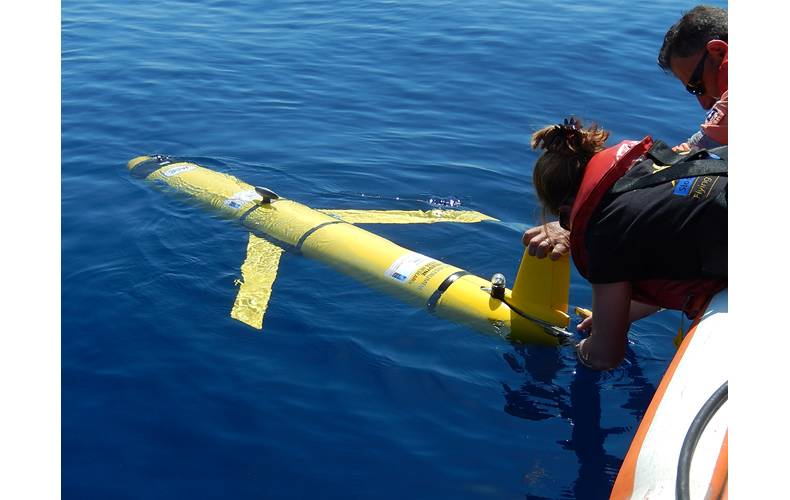
\includegraphics[width=0.8\linewidth]{remus100cmre}
				\caption{REMUS 100 AUV at CMRE: Potential target application}
			\end{figure}
		\end{column}
	\end{columns}
	\vfill
	\centering
	Adoption of open interoperability stds. and ``CoTS'' procurement pipelines

	\centering
	\textbf{Novel and unique threats to trust and security}

\end{frame}

\section{Aims}

\begin{frame}{Open Questions}
		\begin{itemize}
			\item \textbf{Centralised} security difficult/expensive to maintain
			\item Presents \textbf{single-point-of-failure} for operational support
			\item Move from Centralised to Distributed trust management already demonstrated in Terrestrial \textbf{MANETs}
			\item Constrained comms. make comms. only monitoring non-optimal
		\end{itemize}

		\begin{figure}[h]
			\centering
			
\includegraphics[width=0.65\linewidth]{Centralisation}
			\caption{Autonomy is driving increasingly towards distributed applications}
		\end{figure}
	
	\centering
	Can these MANET techniques be applied to the \textbf{marine context}?
	
	\centering
	What metrics can be used to establish and maintain distributed trust?

\end{frame}

\section{Approach}

\begin{frame}{Trust Management in Marine Networks}
	\begin{itemize}
		\item Comms. only Trust Management Frameworks (TMFs) in MANETs
		\item Generally \textbf{Bayesian Estimation} of binary success/fail observation
		\item Not stable in \textbf{sparse, variable, \& noisy} environments
		\item Can (generally) only detect misbehaviour, not classify
		\item Only detects packet-dropping misbehaviours
		\item Recent work uses multiple, continuous, measurements (e.g. \textit{SNR, Delay, Throughput, PLR}) utilising Grey Theory\cite{Guo11} to form a trust ``\textbf{vector}''
		\item Provides \textbf{multi-dimensional classification} of misbehaviour
	\end{itemize}
\end{frame}

\begin{frame}{Novelty}
	\begin{itemize}
		\item \textbf{Assess} existing approaches in simulated UAN, characterising their bounds of suitability/performance
		\item \textbf{Extend} multi-metric approach to encompass \textbf{physical behaviours} as well as comms.
		\item Treat threat surface as a multi-dimensional constraint space, aiming to restrict and protect operations
	\end{itemize}

	\begin{figure}[h]
		\centering
		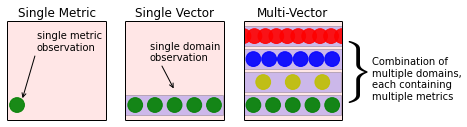
\includegraphics[width=0.65\linewidth]{threat_surface_sum}
		\caption{The available threat surface can be protected through extending trust observations across multiple types of observation}
	\end{figure}
	
\end{frame}
\begin{frame}{Current Results}

	\begin{columns}[T]
		\begin{column}{0.6\textwidth}
			\begin{itemize}
				\item Demonstration of PoC TMF utilising Behavioural Metrics
				\item Protocol for identification/assessment of metric suitability across several misbehaviour types
				\item Performance assessment of Hermes, OTMF, and MTFM in simulated marine environment
				\item Information theoretic assessment of multi-domain combination strategies
			\end{itemize}
			
		\end{column}
		\begin{column}{0.4\textwidth}
			\begin{figure}
				\centering
				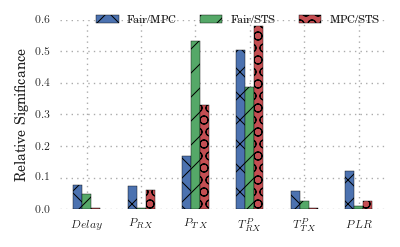
\includegraphics[width=\linewidth]{MaliciousSelfishMetricFactors}
				\caption{Factor Analysis of Malicious, Selfish and Fair behaviours}
				\label{fig:malselfactors}
			\end{figure}
		\end{column}
	\end{columns}
\end{frame}

\section{Impact}

\begin{frame}{Current Outputs}
	\begin{itemize}
		\item Summer Research \textbf{Placement with DSTL} (Software Systems and Dependability for Autonomous Teams/Naval Systems Group)(2013, PDW)
		\item \textbf{Paper} Presentation to the Association for the Advancement of Artificial Intelligence (AAAI) (Stanford, USA) \cite{Bolster2014}
		\item \textbf{Technical Report} for the UK/US/CAN/AUS/NZ Technical Cooperation Programme \cite{Bolster2014a}
		\item DSTL \textbf{CDE Collaboration} with NPL and Plextek Ltd. on ``Precision Timing and Navigation, Resilient Time and Location Estimation for Networked Assets'' (CDE 33135)
		\item \textbf{Paper} Presentation to the IEEE International Symposium on Recent Advances of Trust, Security and Privacy in Computing and Communications (TrustComm, Helsinki, FI) \cite{Bolster2015}
	\end{itemize}
\end{frame}

\begin{frame}{Future Impacts}
	\begin{itemize}
		\item Advisory factor to FF2020 on application \& verifiability of \textbf{in-field autonomy}
		\item Deployment of smaller/cheaper collective assets, through \textbf{lowering comms overheads}
		\item Increase viability / \textbf{confidence} for ``stand-off'' MCM
		\item Increased \textbf{reliability} of autonomous/mixed SoS through continual self-policing
		\item Applications beyond marine; applicable to any constrained / DTN as well as to virtual/\textbf{cyber-physical systems} (i.e. the application of these methods to abstract metric domains)
	\end{itemize}
	
\end{frame}

%
\begin{frame}[t,allowframebreaks]
  \frametitle{References}
  \printbibliography[title=References]% [nottype=video]}
\end{frame}

\begin{frame}
  \centerline{The End}
\end{frame}
% End of slides
\end{document} 


